% Generated by tex/build_swebok_structure.py from tex/chapters/ch01/09_実務上の考慮.tex
\subsubsection{要求の追跡可能性}

\term{追跡可能性}とは、要求がどこから来て、どの設計、コード、テスト、文書につながるかをたどれることです。これは二つの目的で役立つ。

第一に、成果物間の整合性確認である。ある要求に対応する設計要素がなければ、その要求は満たされていない可能性がある。逆に、ある設計要素に対応する要求がなければ、その設計要素は不要か、要求が不足している可能性がある。

第二に、変更の影響分析である。ある要求が変わったとき、関連するソフトウェア要求、設計要素、コード、テストケース、利用者文書をたどることで、変更に必要な作業範囲を見積もりやすくなる。

\begin{figure}[htbp]
\centering
\IfFileExists{swebok_structure/CH01.ソフトウェア要求(Software_Requirements)/1.7.実務上の考慮(Practical_Considerations)/1.7.3.要求の追跡可能性(Requirements_Tracing)/assets/fig-ch01-11.png}{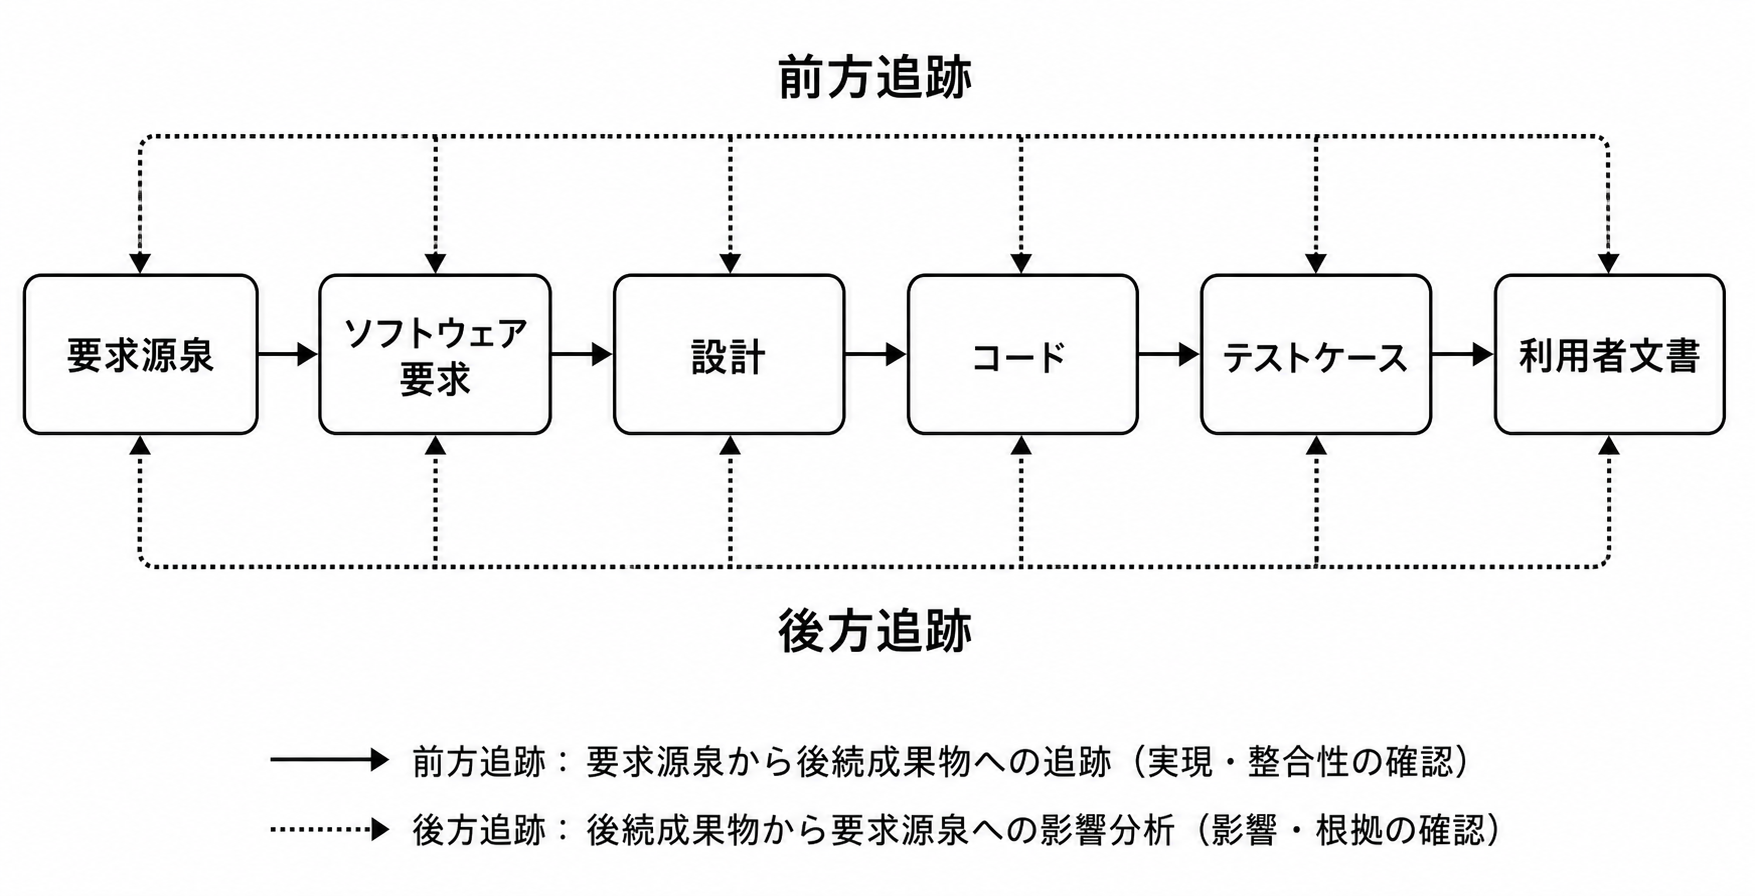
\includegraphics[width=0.96\linewidth]{swebok_structure/CH01.ソフトウェア要求(Software_Requirements)/1.7.実務上の考慮(Practical_Considerations)/1.7.3.要求の追跡可能性(Requirements_Tracing)/assets/fig-ch01-11.png}}{\fbox{\parbox[c][48mm][c]{0.9\linewidth}{\centering 画像生成待ち\\要求追跡の連鎖図}}}
\caption{要求追跡の連鎖図}
\label{fig:ch01-11}
\end{figure}
